\graphicspath{{imgs/}}
\documentclass[main.tex]{subfiles}
\begin{document}
\chapter{Results}\label{chap:results}
This chapter presents the result of the training process. The final network performance is evaluated and compared to other papers. The network's extracted features are further analyzed and a way forward is sketched.

\section{Training Results}
The model performs after training (see Figure~\ref{fig:validation}) with a sensitivity of $81\%$ on the test set. This is already a better result than reported by Xu et al.~\cite{xu1997development}, Armato et al.~\cite{armato1999computerized}, Lee et al.~\cite{lee2001automated}, Suzuki et al.~\cite{suzuki2003massive} and Teramoto et al.~\cite{teramoto2013fast}. But there are also papers that report higher values, like Cascio et al.~\cite{cascio2012automatic} with a sensitivity of $97\%$. I still shows that it is possible to achieve promising results with a pure network architecture.

\begin{figure}
\begin{center}
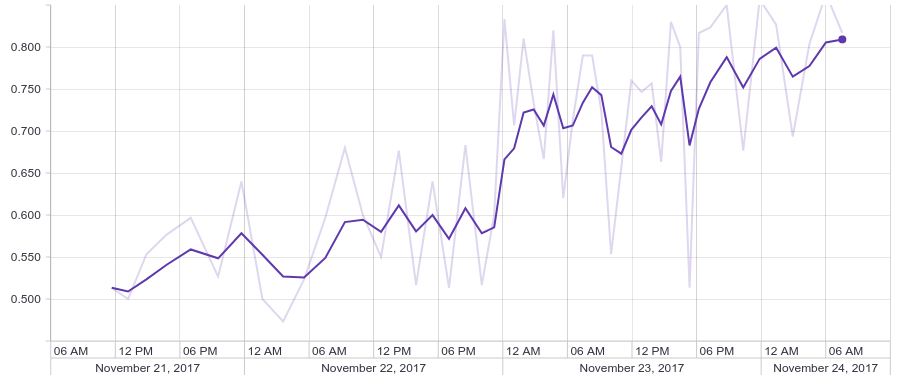
\includegraphics[scale=0.5]{validation_process.png}
\end{center}
\caption{Learning process of the network - the graph shows the development of the accuracy of the network on the validation set. The darker line represents the smoothed values of the lighter line. Since the training is performed on the CPU (GPU can not be utilized since the network was too big.), it takes several days.}
\label{fig:validation}
\end{figure}

There are other metrics to be accounted for though. The false positive rate in the medical context is crucial since the patients suffer under extreme psychological stress if they are to believe that their cancer screening reveals that they are affected by this severe disease. A false positive error can also lead to increased costs connected to additional screening and testing procedures as well as additional health related risks for the patients. The false positive rate of the trained model is $0.19$ per sample, which means that roughly every 5th patch is classified wrongly as being a nodule when it is not. Comparing that to the other approaches is a bit more complex since the reference frame changes. Armato~\cite{armato1999computerized} reports for example a false positive rate of 3 per slice. Given that the used slices in this thesis have a x,y resolution of $512 \times 512$ and the filter kernel is $50 \times 50 \times 5$, this would result in (depending on how the stride is chosen) $100$ patches per $5$ slices. Assuming that the stride would be chosen in a non-overlapping way this would mean a false positive rate of $4$ per slice. This number would rise if the stride would be chosen to jump only one pixel at a time in each direction.  
Considering the practicability of the approach one would also need to measure the time it takes for the algorithm to analyze a complete CT scan.


\section{Analyzing the Network}
The more interesting part besides the performance measure is the question of how the network solves the task. In this section the model architecture will be examined, by running the learning process with different parameters. Then the learned features of the final model will be visualized.


\subsection{Model parameters}
Many decisions concerning the architecture have been made that are not cogent. The choice of the activation function, the number of filters and layers as well as the batch size and other values have been either chosen in the beginning or fixed empirically, because they \emph{worked}. The code structure allows to test easily for the effect of these parameters on the performance. Figure~\ref{fig:other_act} shows the result of a test run with elu activation function~\ref{eq:elu}, which is not so different

\begin{equation} \label{eq:elu}
f(x)= \begin{cases}
    x,& \text{if } x\geq 0\\
    \alpha\left(\exp(x) - 1\right), & \text{if } x\le 0
    \end{cases}
\end{equation}

\begin{figure}
\begin{center}
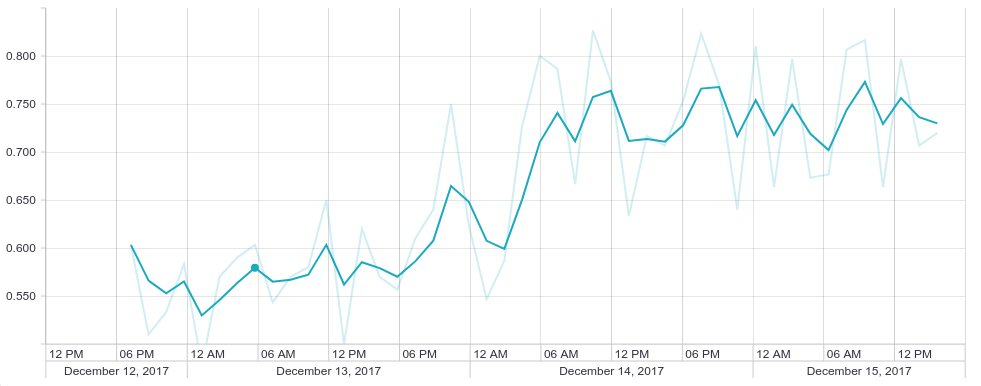
\includegraphics[scale=0.45]{elu_activation.png}
\end{center}
\caption{Another activation function in the dense layers (elu) and in the bottom graph with a batch size of 1.}
\label{fig:other_act}
\end{figure}

A greater impact on the learning has the batch size. The batch size determines how many samples are fed through the network before applying the gradient optimization step. 

\begin{figure}
\begin{center}
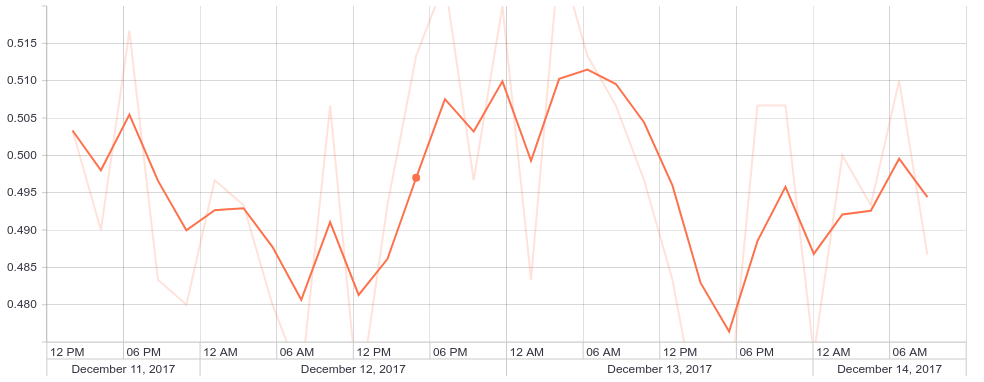
\includegraphics[scale=0.45]{small_batch.png}
\end{center}
\caption{The batch size for this run has been set to 1, decreasing the performance tremendously.}
\label{fig:small_batch}
\end{figure}


\subsection{Learned Features}
To understand how the network solves the task it makes sense to look at the patterns it's layers are sensitive to. The convolutional layers are a suitable target for this kind of inspection, since their activation maps can be directly interpreted by visual inspection, where as the activation of the dense layers does not yield such information straight away. Figure~\ref{fig:mean_activation} shows the mean activation of 4 of the kernels in the first layer after passing through 500 nodule patches. Since the nodules are located in the middle of the input the filters respond to that area. They also show the typical round morphology.


\begin{figure}
\begin{center}
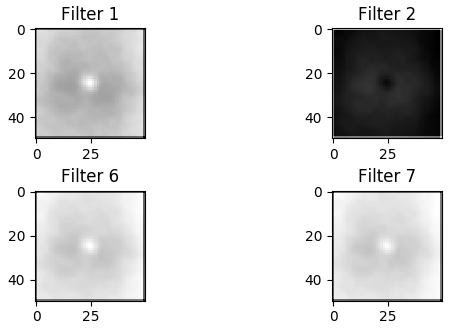
\includegraphics[scale=0.5]{nodule_activation_example.png}
\end{center}
\caption{The mean activation from 500 nodule patches of the validation set. Already in the first layer the receptive field is focusing on the center area, where the nodule resides.}
\label{fig:mean_activation}
\end{figure}


%\section{Bridge to other Approaches}
%At this level of analysis, it seems that the network is leveraging the same morphological features %hat are also used in the hand crafted approaches.


%How could a comparison at all be achieved? What is hindering the straightforward comparison of %the kernel weights? Draw out a method to do that
%Show what has been done
%Compare performance to hand crafted approaches, 
%take numbers out of papers

%what could be similar features in the network?
\end{document}